\documentclass[a4paper, brazil]{article}
\usepackage[utf8]{inputenc}

\usepackage[cm]{fullpage}
\usepackage{pacotesLaTeX}

\author{Thales Freitas Macêdo \\ DRE: 115 162 177}
\title{LISTA 2}

\begin{document}

\maketitle

\section{Exercício 1}

\begin{figure}[ht]
\centering
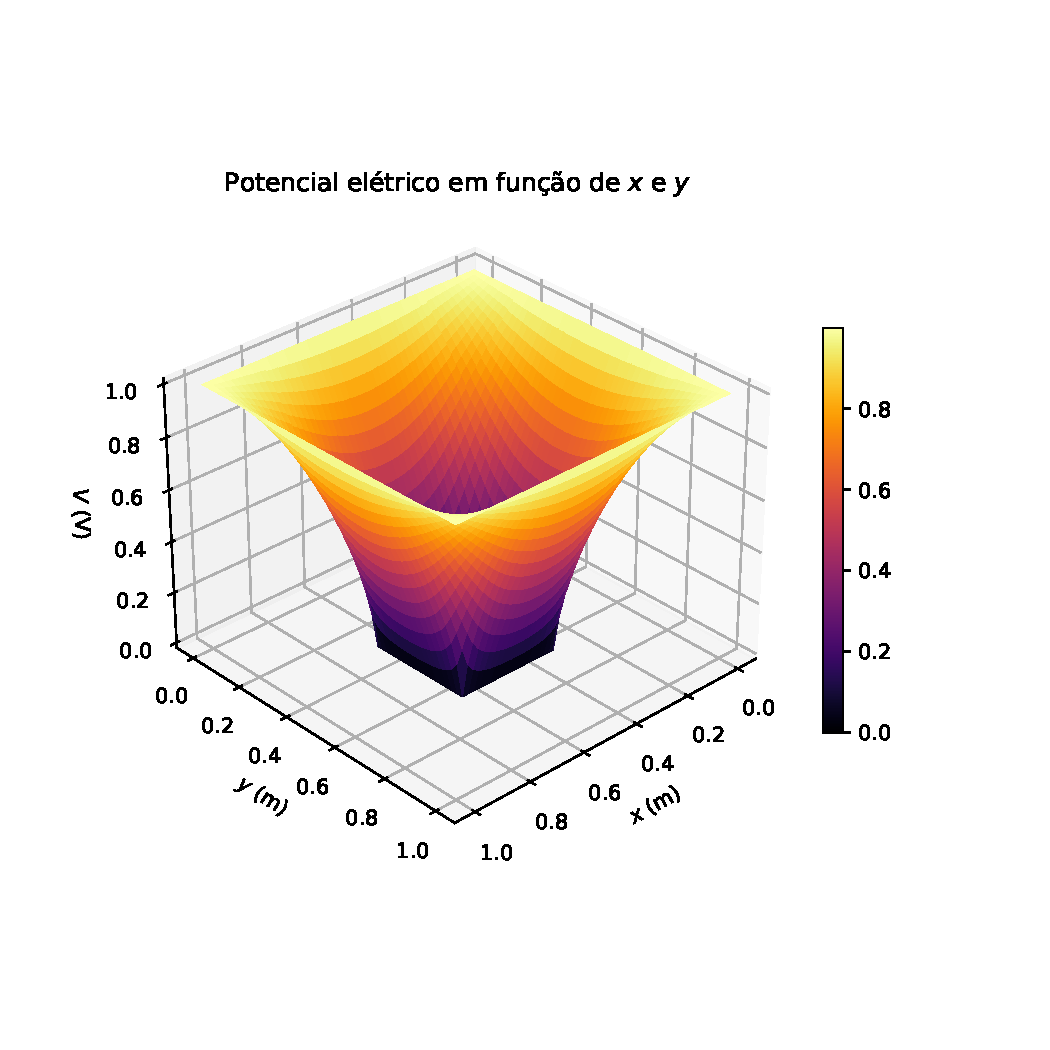
\includegraphics[width=0.4\textwidth]{imagem1_V1.pdf}
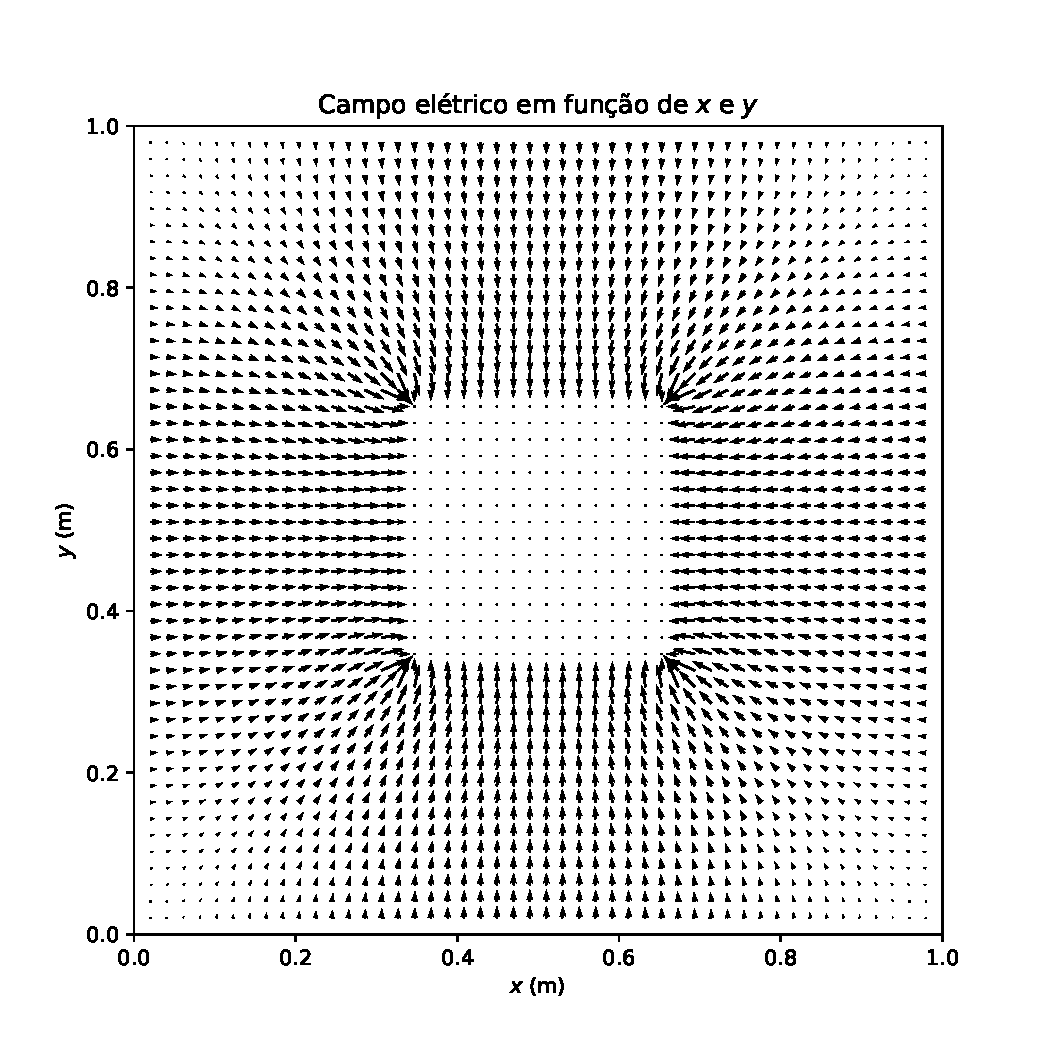
\includegraphics[width=0.4\textwidth]{imagem1_E1.pdf}
\caption{Gráficos do potencial elétrico e do campo elétrico para a configuração do exercício 1.}\label{fig1}
\end{figure}

A figura \ref{fig1} apresenta os gráficos para a configuração  de uma caixa metálica quadrada, de lado \SI{1.0}{\meter}, mantida a um potencial de \SI{1.0}{\volt}, com uma região quadrada interna centralizada de lado \SI{0.36}{\meter}.
Os gráficos apresentam o comportamento esperado pro potencial elétrico que segue a Equação de Laplace.
O gráfico do campo elétrico apresenta um problema nas imediações das condições de contorno, onde a magnitude de \( E \) é muito pequena.
Assim, nesses pontos, os valores encontrados deveriam ser desprezados.

\newpage
\section{Exercício 2}

As dimensões usadas para o exercício foram uma caixa retangular de largura \SI{2.0}{\meter} e altura \SI{1.0}{\meter}.
A placa com potencial \SI{1.0}{\volt} foi colocada na posição \( x = \SI{0.50}{\meter} \) e a placa com potencial \SI{-1.0}{\volt} na posição \( x = \SI{1.50}{\meter} \), ambas com comprimento \SI{0.56}{\meter}.

\subsection{(a)}

\begin{figure}[ht]
\centering
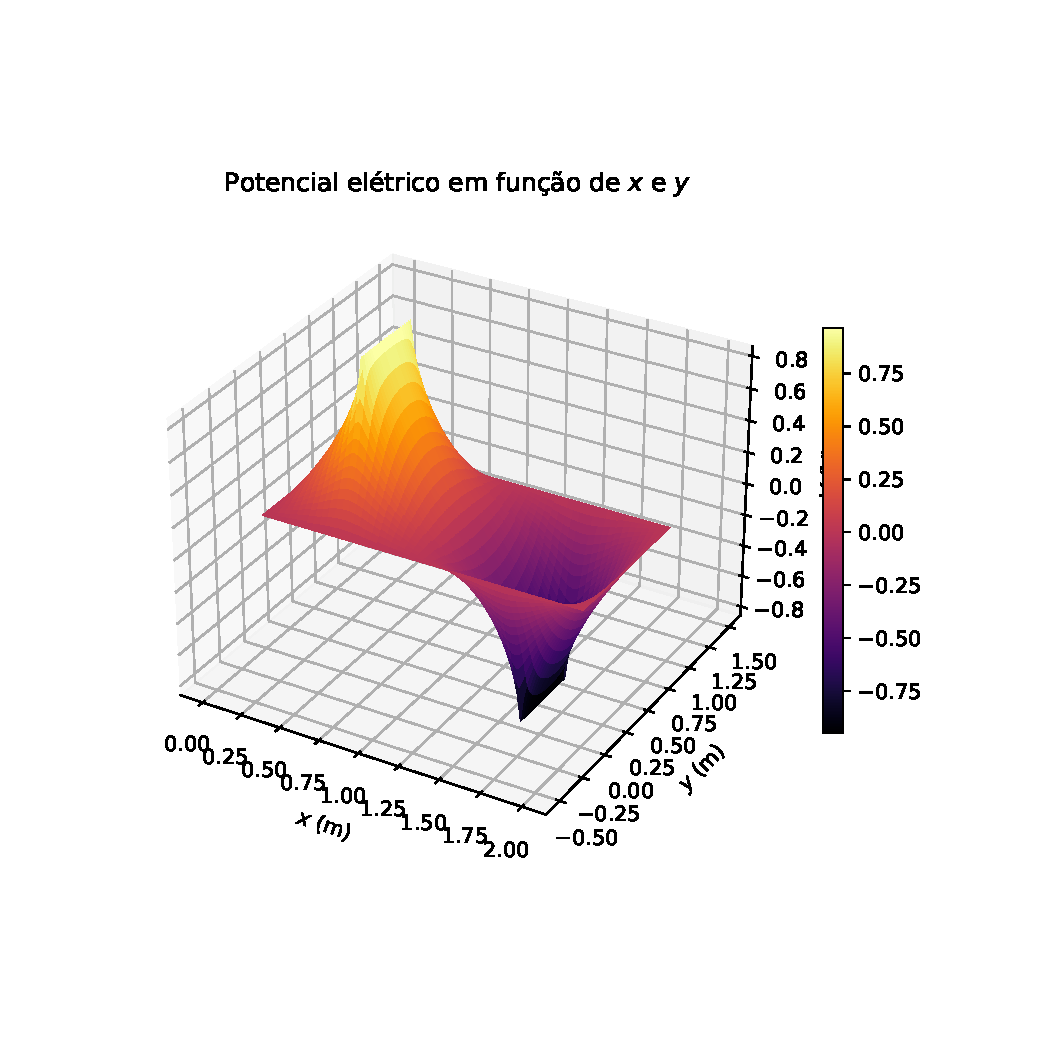
\includegraphics[width=0.4\textwidth]{imagem2_V2.pdf}
\caption{Gráfico do potencial elétrico para a configuração do exercício 2.}\label{fig2a}
\end{figure}

\subsection{(b)}

\begin{figure}[ht]
\centering
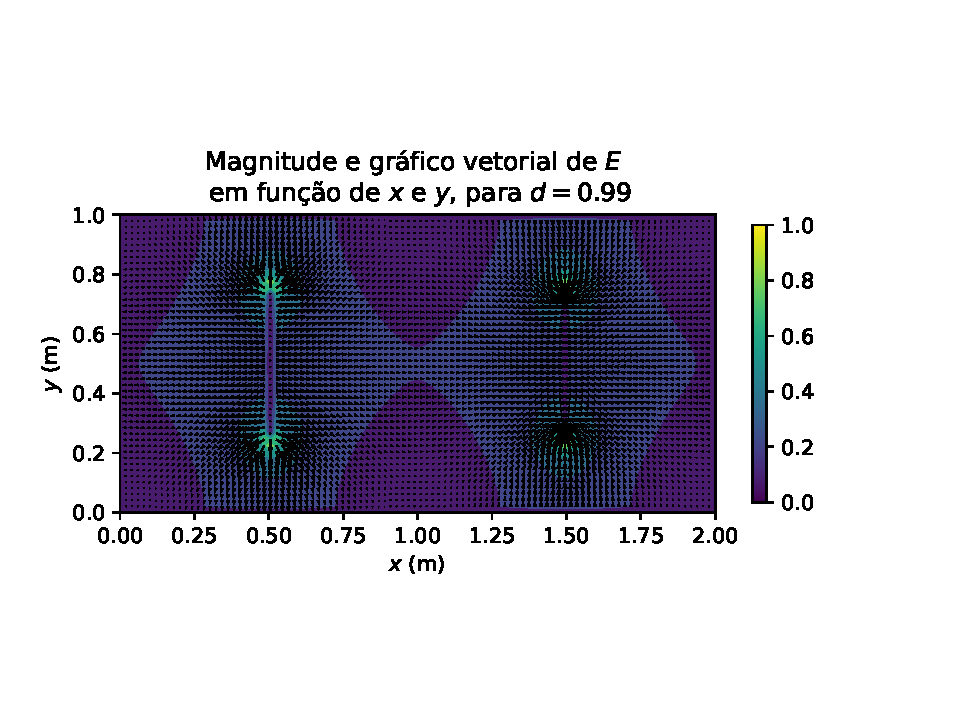
\includegraphics[width=0.4\textwidth]{imagem2_E2.pdf}
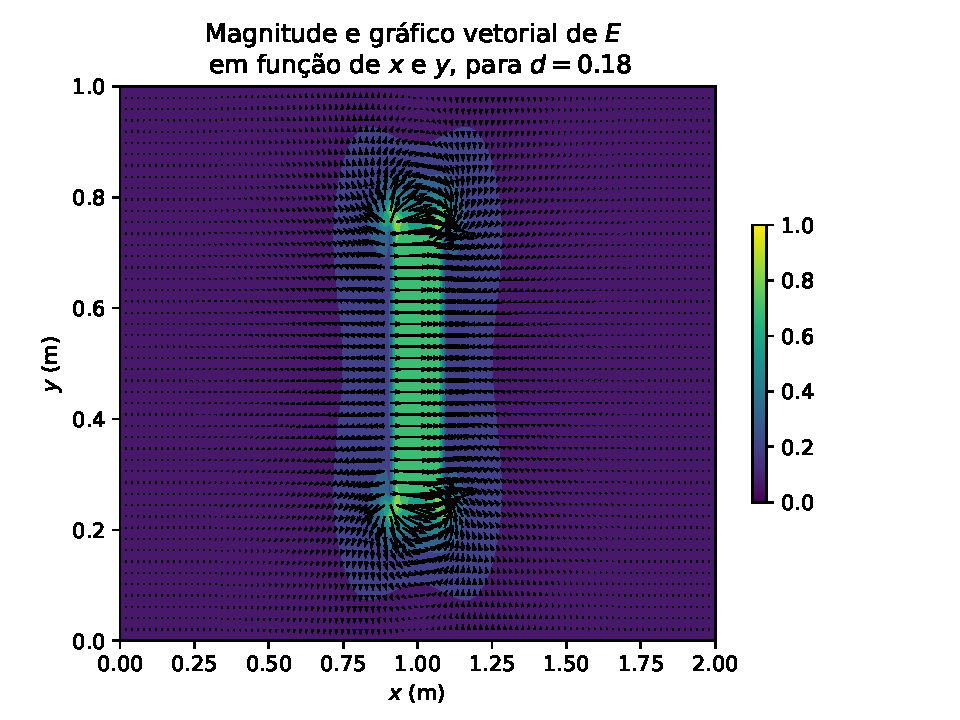
\includegraphics[width=0.4\textwidth]{imagem2_E2b.pdf}
\caption{Gráficos da magnitude e vetorial de \( E \), com diferentes distâncias entre as placas.}\label{fig2b}
\end{figure}

\subsection{(c)}

Quando as placas estão mais separadas em comparação com os seus comprimentos, as bordas se comportam como fontes ou sumidouros de campo elétrico.
Quando as placas estão a uma distância pequena em comparação com os seus comprimentos, o campo contorna as bordas das placas.

\newpage
\section{Exercício 3}

\begin{figure}[ht]
\centering
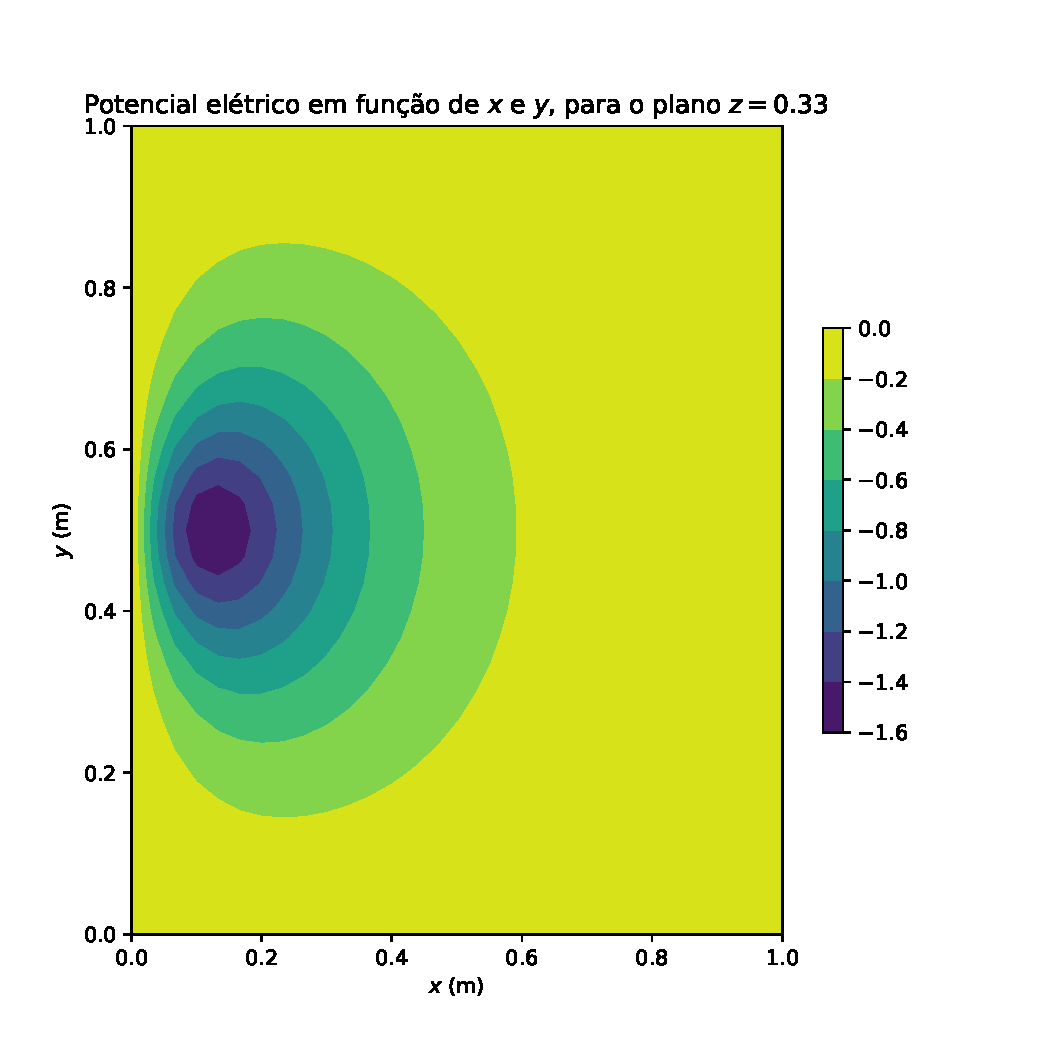
\includegraphics[width=0.7\textwidth]{imagem3.pdf}
\caption{Gráfico do potencial elétrico de uma seção \( xy \) do cubo do exercício 3.}\label{fig3a}
\end{figure}

Para o exercício 3, a carga puntiforme de \SI{- 1.0}{\coulomb} foi colocada na posição \( x = \SI{0.07}{\meter} \), \( y = \SI{0.5}{\meter} \) e \( z = \SI{0.5}{\meter} \), de um cubo de lados \SI{1.0}{\meter}.
Podemos ver que as curvas equipotenciais formam curvas ovaladas, que se concentram mais próximas à face da carga puntiforme.

%\newpage
\section{Exercício 4}

Os arquivos dos vídeos serão enviados em anexo no e-mail.
Para \( r = 1 \), o vídeo 1 mostra o pulso sendo refletido pelo mesmo lado da corda, ao contrário do caso de pontas fixas.

Para \( r = 0.1 \), no vídeo 2, é possível ver que conforme o tempo passa o pulso começa a diferir do vídeo 1, mostrando que os erros associados ao método numérico se acumulam ao longo do tempo.

Para \( r = 2 \), no vídeo 3, o pulso explode rapidamente, claramente divergindo do resultado esperado.
Esse caso é inadequado para a resolução do problema devido à sua alta instabilidade.

\end{document}
